\begin{frame}
  \frametitle{Model}
    \begin{columns}
        \column[t]{5cm}
            \begin{itemize}
                \item 2 $\times$ 2 asymmetrical pincell lattice
                \item Two materials (UO2, H2O), 7 energy groups, six delay
                    groups
                \item Radial and azimuthal (not pictured) discretization for
                    fuel, 10 $\times$ 10 mesh discretization for all-water region
                    (not pictured)
            \end{itemize}
        \column[t]{5cm}
            \begin{figure}[htbp!]
                \begin{center}
                    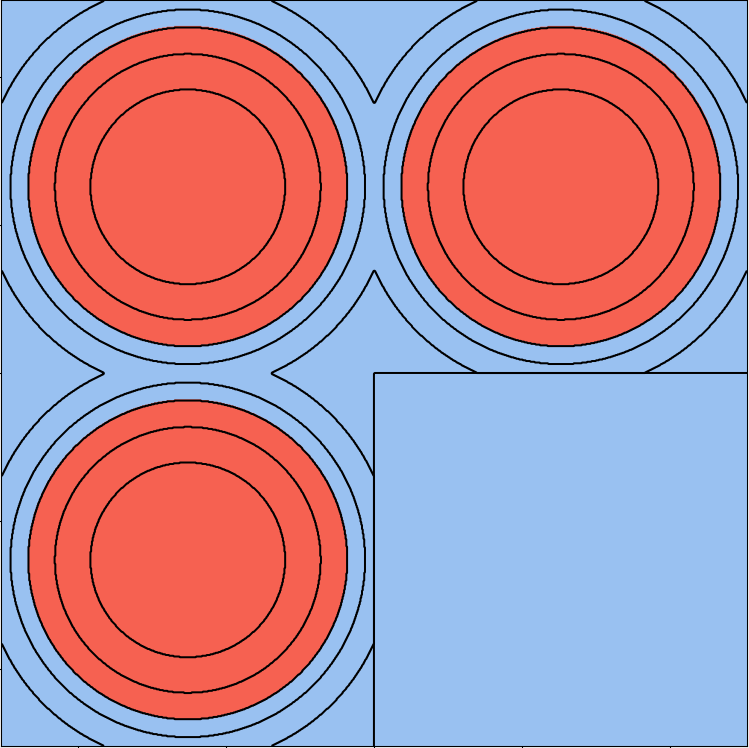
\includegraphics[height=4cm]{./figs/geometry-cells.png}
                \end{center}
                \caption{Problem geometry, pink is UO2 fuel, blue is H2O
                moderator, black lines show cell boundaries (azimuthal and mesh
                lines not shown)}
                \label{fig:geometry}
            \end{figure}
        \end{columns}
\end{frame}

\begin{frame}
  \frametitle{Proposed transient}

  Using the pyXSteam package, calculate a timeseries of H2O densities in
  20 steps from 
  580K to 620K and back to 580K assumeing a constant pressure of 16MPa.
  Apply the density change to the water-only region of the model.
\end{frame}


